\documentclass[11pt]{beamer}                                                                                                   %\usetheme{Madrid}
\usepackage{graphicx}
\usepackage{subfigure}
\usepackage[english]{babel}
\usepackage{times}
\usepackage{caption}
\usepackage[T1]{fontenc}
\usepackage{ctex}
%\usepackage{beamerthemesplit} % 加载主题宏包
\usetheme{Warsaw} % 选用该主题
%\useinnertheme{default} % 选用该主题
\usepackage{multicol}


% 设置页码的外观和位置
\setbeamertemplate{page number in head/foot}[framenumber] % 显示幻灯片页码
\setbeamertemplate{footline}[frame number] % 显示页码在底部导航栏
\begin{document}
	%\begin{frame}
	\title[Paper Summary]{Sherman: A Write-Optimized Distributed B+Tree Index on Disaggregated Memory,  
		   
		
		
	Qing Wang, Youyou Lu, Jiwu Shu∗


SIGMOD22  }
	\author[report]{Reporter: Luo Tianyi} % 显示作者
	\institute[Luo Tianyi]{Koukou, HUST} % 设置学院机构
	\date{\today}  % 显示日期
	\logo{
\includegraphics[width=2.1cm,height=1.5cm]{1.png}}
	\begin{frame}
		\titlepage
	\end{frame}
%\section[Contents]{}
%%%%%%%%%%%%%%%%%%%%%%%%%%%%%%%%%%%%%%%%%
\begin{frame}
	\frametitle{Contents}
	\begin{multicols}{2}
		\tableofcontents
	\end{multicols}
\end{frame} 
%\AtBeginSubsection[] {
%	\frame<handout:0> {
%		\frametitle{Contents}
%		\tableofcontents[current,currentsubsection]
%	}
%}
\section{Background}
\subsection{RDMA}
\begin{frame}
	\frametitle{Background : RDMA}
	\begin{columns}
		\begin{column}{0.5\textwidth}
			\centering
			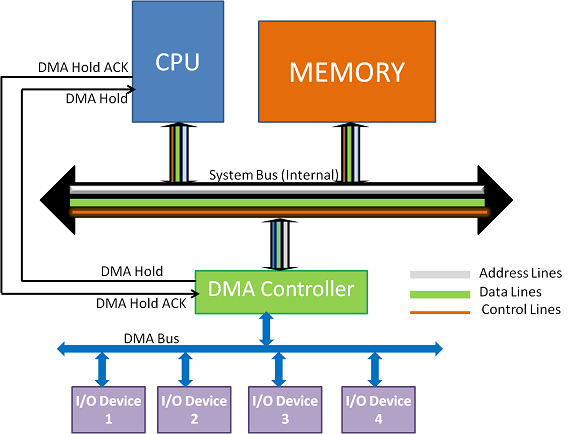
\includegraphics[height=3.5cm]{00.png}
			\\
			{DMA Ideas}
		\end{column}
		\begin{column}{0.5\textwidth}
			\centering
			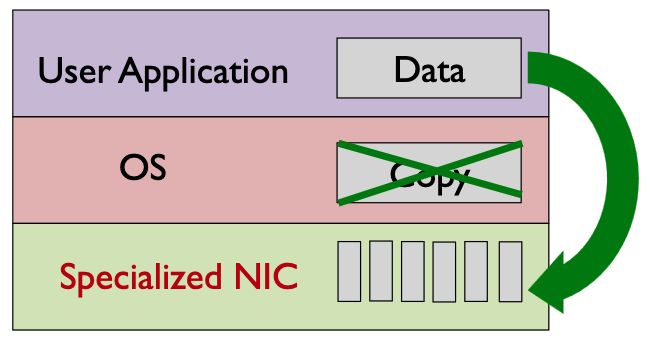
\includegraphics[height=3.5cm]{01.png}
			{RDMA Ideas}
		\end{column}
	\end{columns}
		%\begin{figure}[ht]%%图
		%	\centering  %插入的图片居中表示
%			
%			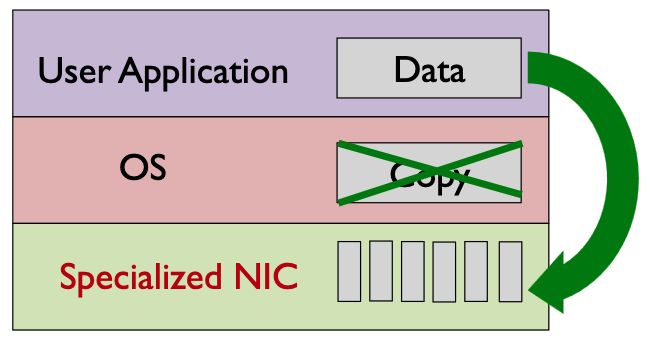
\includegraphics[width=0.5\textwidth]{01.png}  
%			\caption{Design Ideas Of RDMA}  %图片的名称
			

%	\end{center}
\begin{itemize}
%	\item Remote Direct Memory Access : From DMA
	\item DMA->RDMA Reduce the number of copies, reduce CPU involvement, and support remote access.
	\item One-Sided and Two-Sided verbs
	\item {Specialized NICs and communication protocols, 
	
	
	developing to ultra-fast access}
\end{itemize}

\end{frame}



\begin{frame}[t]
	
\begin{columns}
		\begin{column}{0.4\textwidth}
			\centering
			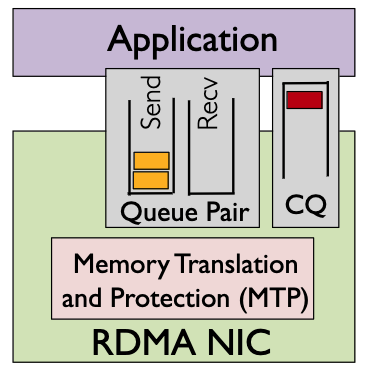
\includegraphics[height=3.5cm]{03.png}
			\\
			{OS Bypass}
		\end{column}
		\begin{column}{0.6\textwidth}
			\centering
			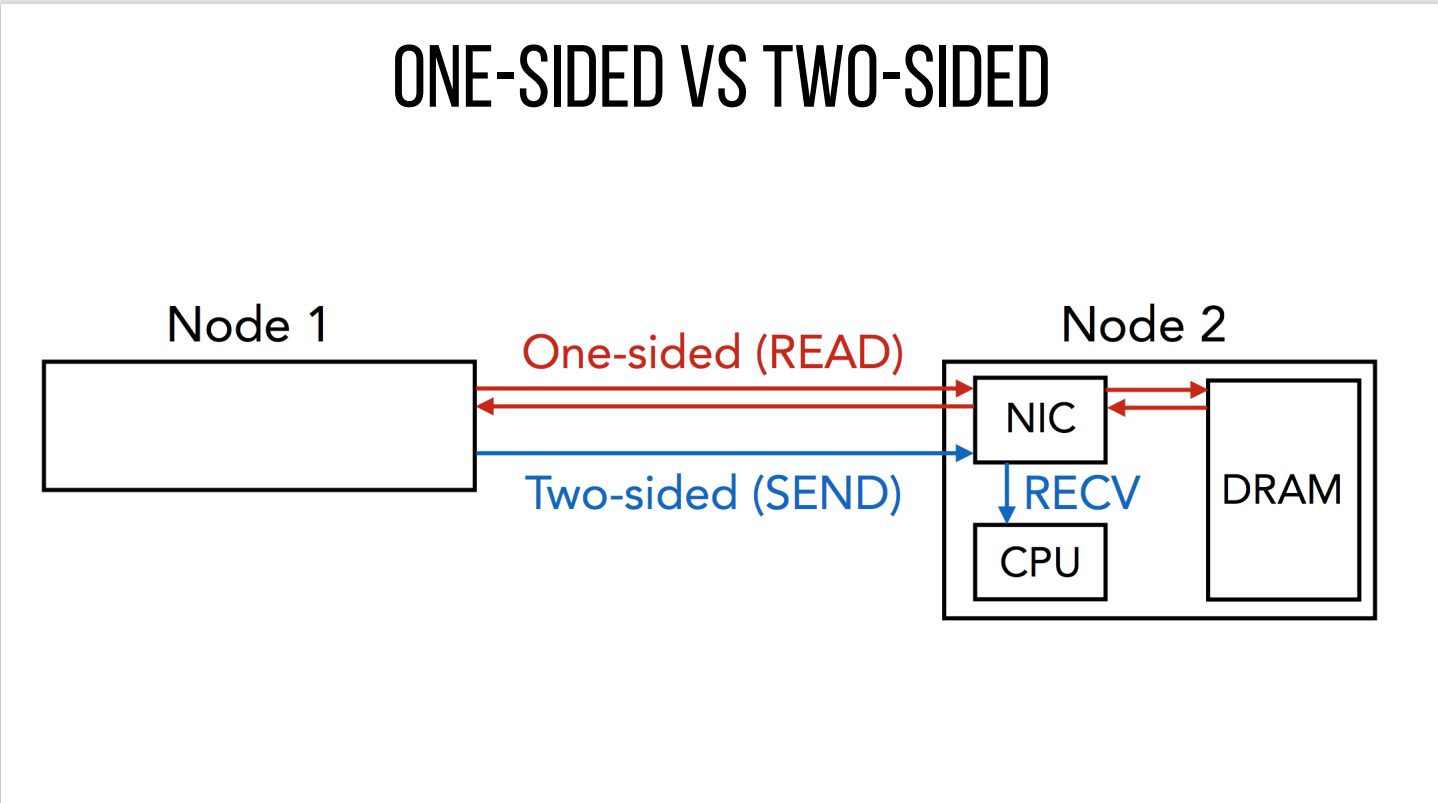
\includegraphics[height=3.5cm]{04.png}
			{Verbs}
		\end{column}
	\end{columns}

		\begin{itemize}
			\item Two-Sided: pass control messages
			\item One-Sided: Memory copy
			\item Verbs: int ibv\_post\_send(struct ibv\_qp *qp, struct ibv\_send\_wr *wr, struct ibv\_send\_wr **bad\_wr);
		\end{itemize}
%	\end{center}
\end{frame}

\begin{frame}[t]
	
	\begin{figure}[ht]%%图
		\centering  %插入的图片居中表示
		%			
		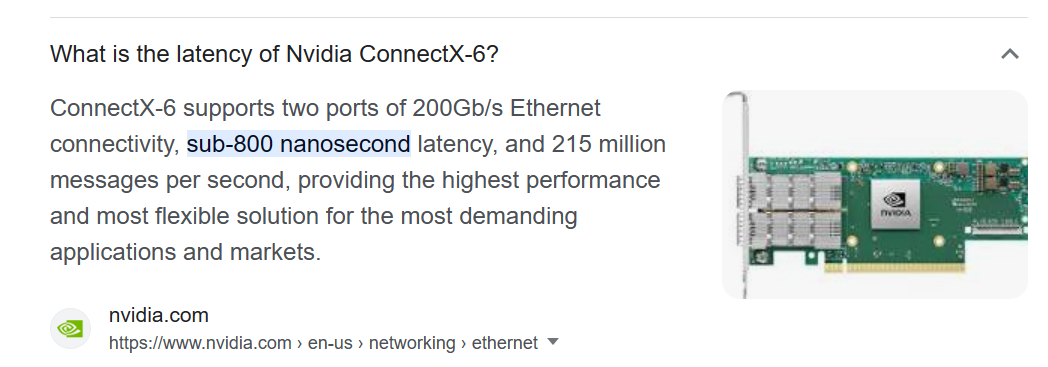
\includegraphics[width=0.88\textwidth]{02.png}  
		\caption{RDMA NICs Performance}  %图片的名称
		
	\end{figure}
	\begin{itemize}
		\item Microsecond level latency and high bandwidth
		\item Available for disggregated design
	\end{itemize}
	%	\end{center}
\end{frame}
%\begin{frame}[fragile]
%	\frametitle{Pearson Correlation}
%	\begin{figure}[t]%%图
%		\centering  %插入的图片居中表示
%		
\includegraphics[width=\textwidth]{1.png}  
%		\caption{Pearson Correlation Heatmap}  %图片的名称
%	\end{figure}
%\end{frame}
\subsection{Disaggregated Memory}
\begin{frame}[t]
	\frametitle{Background : Disaggregated Memory}
		\begin{figure}[ht]%%图
		\centering  %插入的图片居中表示
		%			
		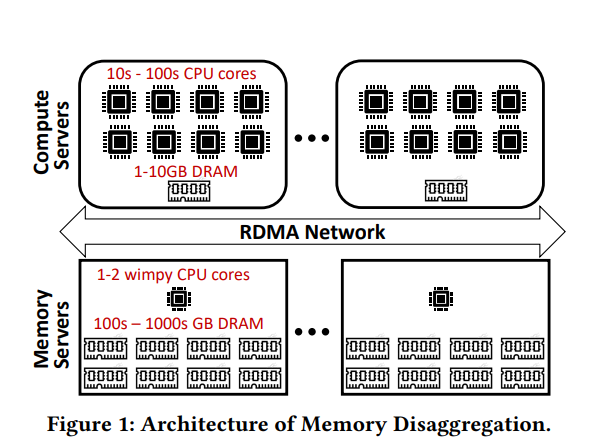
\includegraphics[width=0.60\textwidth]{05.png}  
		
	\end{figure}
\begin{itemize}
	\item Resource disggregation
	 : Near zero computer power on memory side
\end{itemize}
\end{frame}

\subsection{B+Tree Index Structure In DB}
\begin{frame}[fragile]
	\frametitle{Background : B+ Tree}
	Index Structure: A key technique to speed up massive data query, Determing the performance of DB system
	
	B+ Tree Index: A widely-used tree index in DB systems, support range query...
			\begin{figure}[ht]%%图
		\centering  %插入的图片居中表示
		%			
		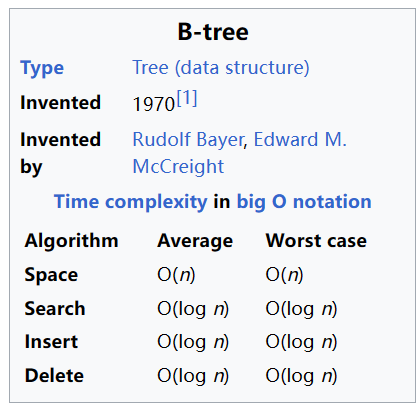
\includegraphics[width=0.5\textwidth]{06.png}  
		
	\end{figure}
\end{frame}
\begin{frame}[t]
	Basic structure of B+Tree:
	\begin{figure}[ht]%%图
		\centering  %插入的图片居中表示
		%			
		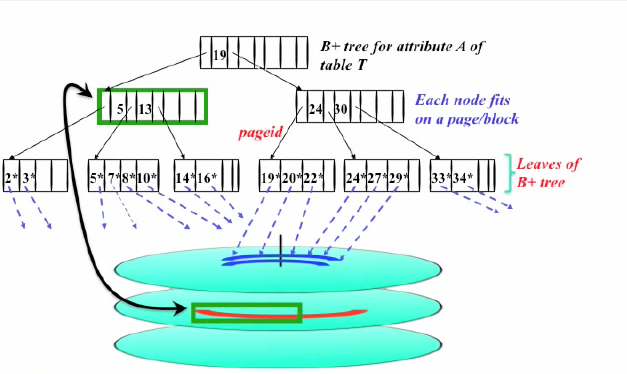
\includegraphics[width=0.60\textwidth]{07.png}  
		
	\end{figure}

		\begin{itemize}
		\item Fast read(query)
		\item Relatively slow write(insert)
	\end{itemize}
\end{frame}
\section{Bottleneck}
\subsection{Existing Approaches}
\begin{frame}[fragile]
	\frametitle{Bottleneck : Existing Approaches}
	No previous design on disggregated memory.
	
	(1) Using One-sided Verbs Purely, FG
		\begin{figure}[ht]%%图
		\centering  %插入的图片居中表示
		%			
		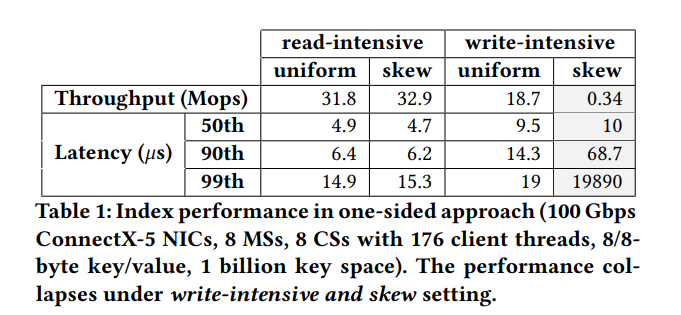
\includegraphics[width=0.7\textwidth]{08.png}  
		
	\end{figure}
\end{frame}
\begin{frame}[t]
	No previous design on disggregated memory.
	
	(2) Extending RDMA Interfaces
	\begin{figure}[ht]%%图
		\centering  %插入的图片居中表示
		%			
		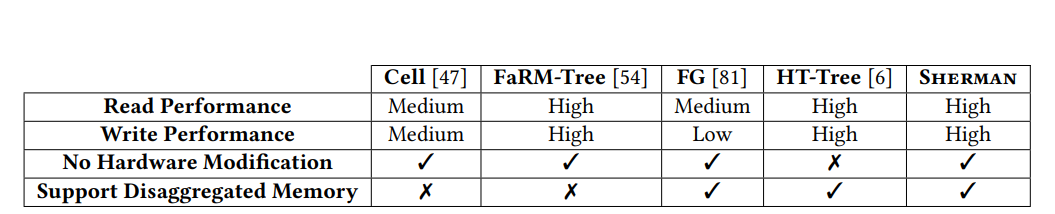
\includegraphics[width=1\textwidth]{09.png}  
		
	\end{figure}
			\begin{itemize}
		\item Hard to deploy
	\end{itemize}
\end{frame}

\subsection{Slow Write Operations}
\begin{frame}[t]
	\frametitle{Bottleneck : Slow Write Operations}
	Reasons?
	(1) Excessive Round Trips when modifying a Tree node.
	
	
	What's RTT?
	
	
	Round-trip time (RTT) is the duration in milliseconds (ms) it takes for a network request to go from a starting point to a destination.
	
	
	
	\vspace{1cm}
	  
	  
	  
	A client thread needs 4 round-trips: 
	
				\begin{itemize}
		\item Acquiring associated exclusive lock
		\item Reading the tree node, 
		\item Writing back the modified tree node
		\item And finally releasing the lock
	\end{itemize}  
\end{frame}
\begin{frame}[t]
	(2) Slow Synchronization Primitives
	
	\begin{itemize}
		\item Expensive in-NIC concurrency control
			\begin{figure}[ht]%%图
			\centering  %插入的图片居中表示
			%			
			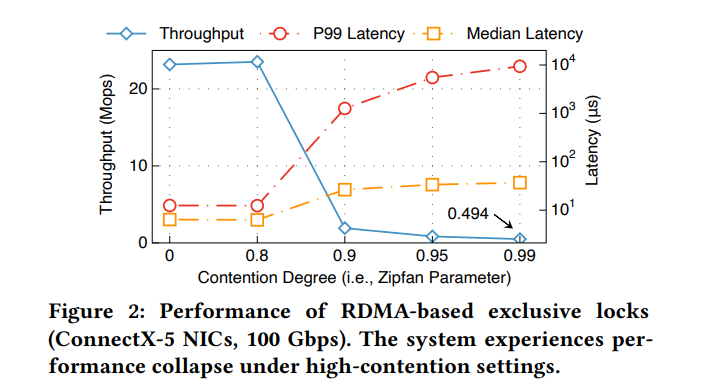
\includegraphics[width=0.7\textwidth]{10.png}  
			
		\end{figure}
		\item Unnecessary retries.
		\item Lacking Fairness.
		
	\end{itemize}  


\end{frame}
\begin{frame}[t]
	(3) Write Amplification
	
	\begin{itemize}
		\item Sorted layout: a lot to modify via RDMA\_WRITE
		\item too large I/O size
		\begin{figure}[ht]%%图
			\centering  %插入的图片居中表示
			%			
			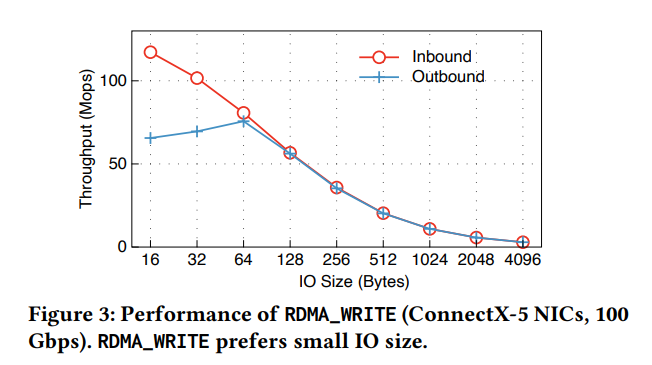
\includegraphics[width=0.7\textwidth]{11.png}  
			
		\end{figure}

		
	\end{itemize}  
	
	
\end{frame}
\section{Design of Sherman}
\subsection{Overview}
\begin{frame}[t]
	\frametitle{Design: Overview}
\begin{figure}
	\centering
	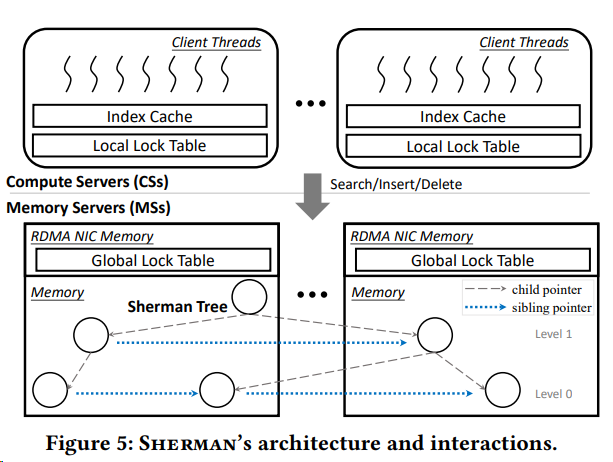
\includegraphics[width=0.7\linewidth]{15}

\end{figure}

\end{frame}
\begin{frame}[t]
	\begin{itemize}
		
	\item Concurrency Control:
	
	Before modifying a tree node, the
	client thread must acquire the associated exclusive lock
	
	
	Use a HOCL approach.
	
	
	\item Cache Mechanism: 
	
	
	Case 1:
	
	
	Internal nodes visited before.  
	
	
	
	Case 2:
	
	
	The first 2 levels of nodes
	
	

	
	
\end{itemize}  

	
\end{frame}
\subsection{Combine}
\begin{frame}[fragile]
	\frametitle{Design : Combine(Reduce RTTS)}
	Abstract: Combine several commands together to reduce round trips.
	
	Case 1:
	
	
		Since a tree node and its lock co-locate at the same Memory node, transmit them together.
		
		
	Case 2:
	
		
		When split and the generated sibling node is in the same Memory node, transmit them together.
\end{frame}


\subsection{Hierarchical On-Chip Lock}
\begin{frame}[t]
	\frametitle{Design : Hierarchical On-Chip Lock(Deal with concurrency control)}
	HOCL leverages on-chip memory of
	NICs to avoid PCIe transactions at MS-side; it also maintains local
	locks at CS-side, to form a hierarchical structure, reduce retries.
	\begin{itemize}
		\item Memory Side: On-chip(NICs) lock table
		\item Compute Side: A local lock table to coordinate conflicting lock requests within the same Compute nodes.
	\end{itemize}  
\end{frame}

\subsection{Two Level Design}

\begin{frame}[t]

	\frametitle{Design : Two Level Design(Deal with the write amplification)}
	\begin{figure}
		\centering
		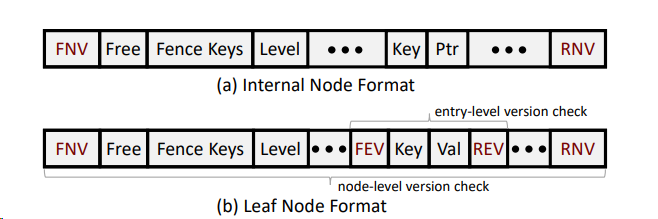
\includegraphics[width=0.7\linewidth]{16}
	\end{figure}
\centering
	Use a version check to control:
	
	
	When not splitting a node, only transmit a 4-bit "version"
\end{frame}
\section{Performance}
\subsection{Exp Setup}
\begin{frame}[t]
	\frametitle{Performance : Exp Setup}
	(1) Hardware
	\begin{figure}
		\centering
		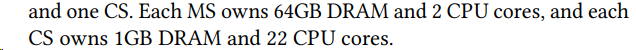
\includegraphics[width=1.0\linewidth]{12}
	
	\end{figure}
	MS: Memory Server
	CS: Compute Server 
	
	
	(2) Workload
	
	
	There are two types of key popularity: uniform and skewed. In uniform workloads, all keys have the same probability of being accessed. Skewed workloads follow a Zipfian access distribution, common in production environments.
	
	(3) Evaluation Indicators
	
	
	Bandwidth and Latency.
\end{frame}

\subsection{Performance Test}
\begin{frame}[t]
	\frametitle{Performance : Performance Test}
	\begin{figure}
		\centering
		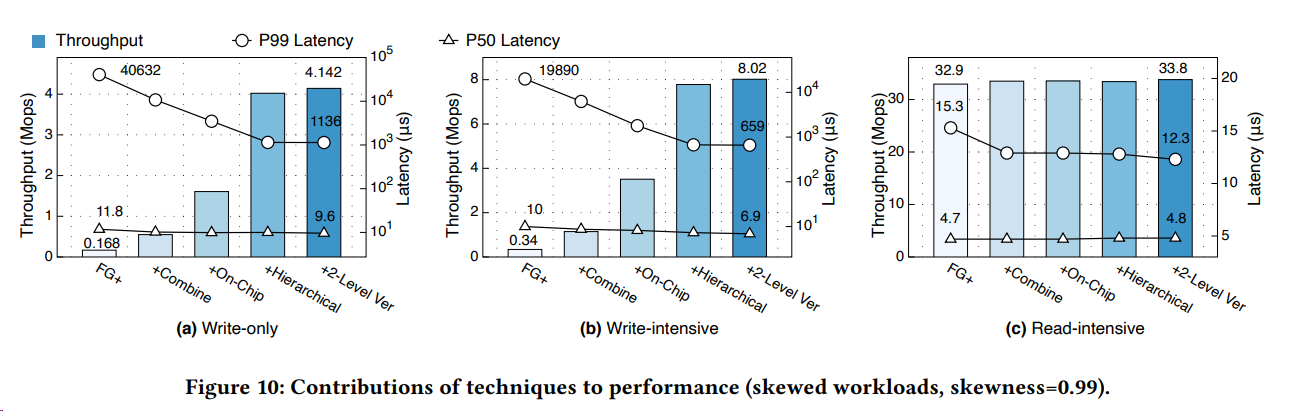
\includegraphics[width=0.9\linewidth]{13}
		
	\end{figure}
	\begin{figure}
		\centering
		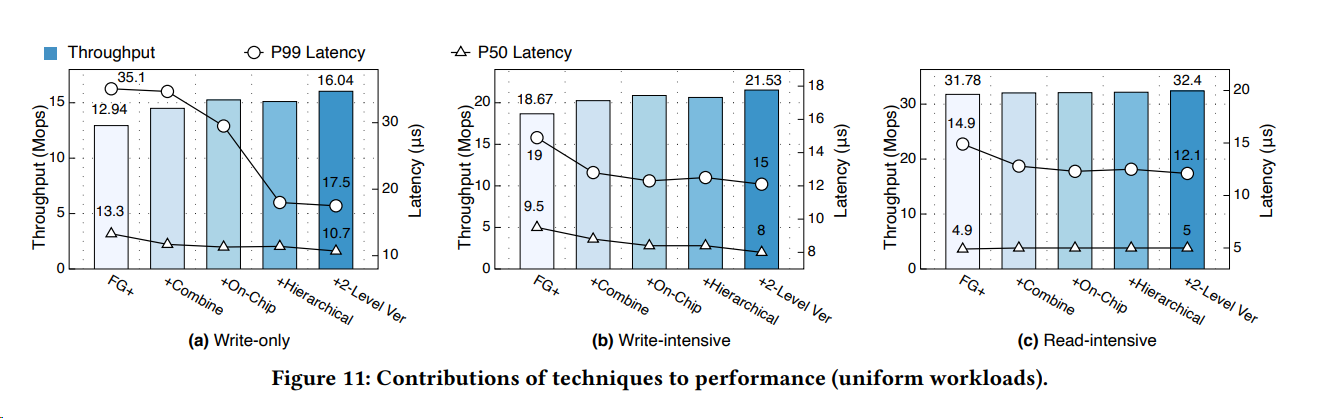
\includegraphics[width=0.9\linewidth]{14}
	\end{figure}
	
\end{frame}

\subsection{Conclusion}
\begin{frame}[fragile]
	\frametitle{Performance : Conclusion}
	The paper proposed and evaluated Sherman, an RDMA-based B+Tree(and the first)
	index on disaggregated memory. Sherman introduces a set of techniques to boost write performance and outperforms existing solutions, demonstrates that combining RDMA
	hardware features and RDMA-friendly software designs can enable
	a high-performance index on disaggregated memory.
\end{frame}
\begin{frame}[plain,c]
	\begin{center}
		\Huge Thank You !
		
		\vspace{2cm}
		\small Luo Tianyi
	\end{center}
\end{frame}
\end{document}